%%MEETING

Scenario = Context + Context Actions (Events)

Context Actions can be defined as:

CtxAct={memberFailure, sensorFailure, envChange, addTask}

x = memberFailure ; y=sensorFailure; z=envChange; w=addTask

CtxAct={x,y,z,w}=x+y+z+w+1 (at least 1 event)

Considering the context: E, M, env(sensors) and initial $C2_{ap}$ 

Let's write CtxAct in terms of Ctx (just to have a reference)

x = E - 1 (only one member remains)
y = 5E (maximum of 5 sensors per member)
z = 5E (envChange causes sensors' modification)
w = E.M (each member can receive a new mission at the same size)

CtxAct = (E-1)+5E+5E+EM+1
CtxAct = E(11+M) 

As resilience($\rho$) returns a function of Scenario,

$\rho = f(Context, CtxAct)$

Resilience = Effectiveness(Scenario)

\begin{figure}
    \centering
    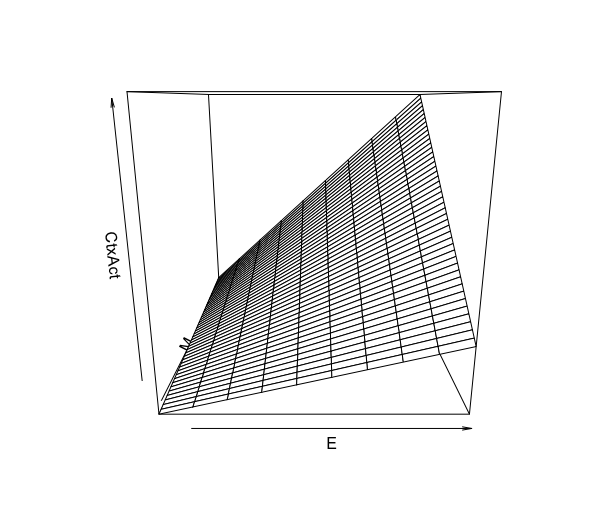
\includegraphics[width=1.0\linewidth]{tex/Rplot.png}
\end{figure}